\documentclass[../main.tex]{subfiles}

\begin{document}

    \subsection{Pokrycia logiczne}

    \begin{figure}[H]
        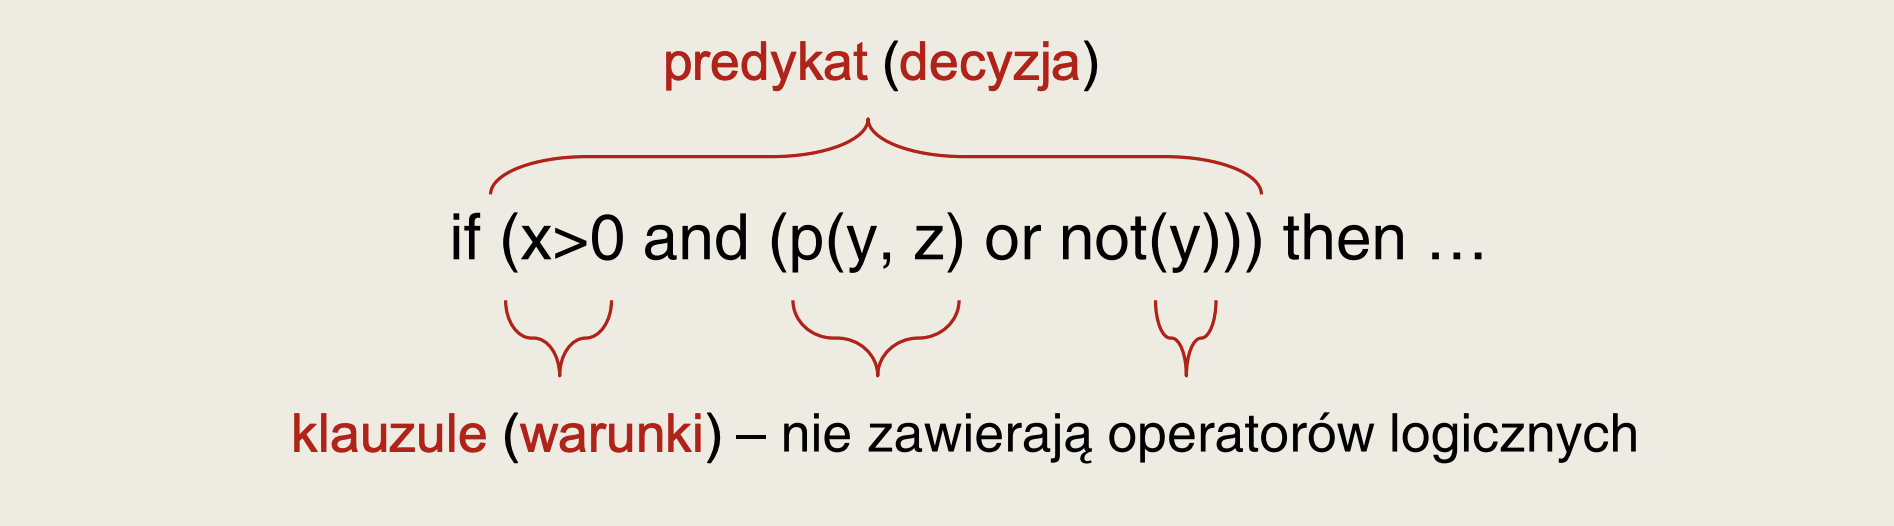
\includegraphics[width=\linewidth]{logika.png}
    \end{figure}

    Predykat może zawierać:
    \begin{itemize}
        \item stałe i zmienne logiczne
        \item wyrażenia porównywane operatorami relacyjnymi
        \item wywołania funkcji
    \end{itemize}

    \subsubsection{Podstawowe kryteria}

    \textbf{Testowanie decyzji} - każda \textbf{decyzja} musi \textbf{przynajmniej raz} przyjąć wartość TRUE i
    przynajmniej raz FALSE.

    Pokrycie decyzji a pokrycie krawędzi
    \begin{itemize}
        \item praktycznie to samo; subtelna różnica dotyczy miary pokrycia
        \item 100\% pokrycia decyzji = 100% pokrycia krawędzi (dlaczego?)
        \item dla niższych stopni pokrycia mogą wystąpić różnice
    \end{itemize}


    \textbf{Testowanie warunków}
    \begin{itemize}
        \item testowanie decyzji rozważa decyzję jako niepodzielną całość
        \item testowanie warunków rozważa sposób ewaluacji decyzji
        \item \textbf{każdy warunek} musi \textbf{przynajmniej raz} przyjąć wartość TRUE i przynajmniej raz wartość FALSE
    \end{itemize}



    \textbf{Testowanie wielokrotnych warunków}
    \begin{itemize}
        \item wymaga przetestowania wszystkich możliwych kombinacji wartości
        logicznych warunków tworzących decyzję
        \item wada: liczba testów jest wykładnicza względem liczby różnych
        warunków: dla N warunków musi być $2^N$ testów
    \end{itemize}

    Jeśli zachodzi \textbf{zwarcie} (short-circuiting), liczba rzeczywistych testów może być zazwyczaj zredukowana.


    \textbf{Subsumpcja kryteriów.}
    \begin{figure}[H]
        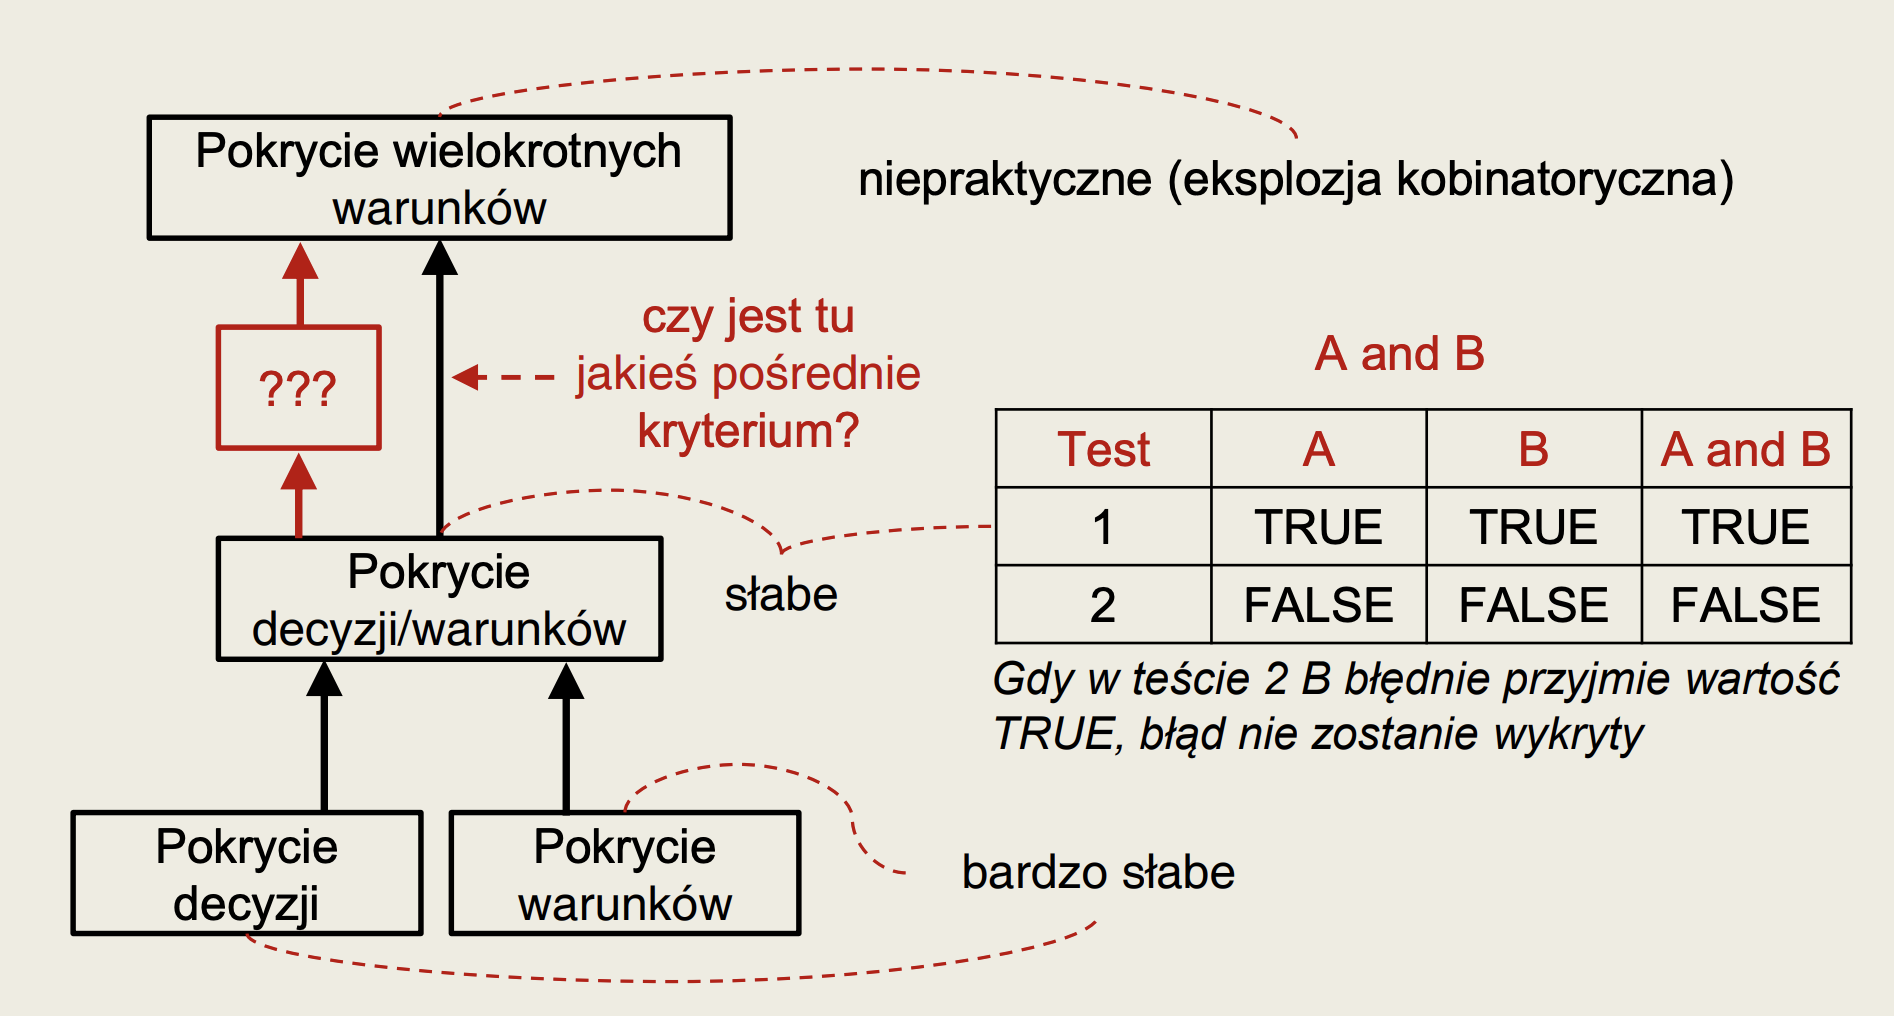
\includegraphics[width=\linewidth]{kryteria.png}
    \end{figure}

    \subsubsection{Kryterium MC/DC}

    \begin{itemize}
        \item zmodyfikowane kryterium warunków/decyzji
        \item słabsze niż wielokrotne warunki, ale silniejsze od warunków/decyzji
        \item dla \textbf{N} warunków wymaga zazwyczaj \textbf{N+1} testów (a więc liniowo)
        \item \textbf{wymaga dostarczenia takich testów, by każdy warunek pokazywał niezależnie swój wpływ na zmianę warunku
        logicznego decyzji}, tzn. dla każdego warunku W w decyzji D muszą istnieć 2 testy:
        \begin{itemize}
            \item W jest TRUE w jednym z nich i FALSE w drugim
            \item D jest TRUE w jednym z nich i FALSE w drugim
            \item wartości logiczne pozostałych warunków w tych dwóch testach
            nie zmieniają się
        \end{itemize}
        \item warunek W dla tych dwóch testów nazywany jest \textbf{klauzulą aktywną},
        a pozostałe warunki – \textbf{klauzulami pobocznymi}
    \end{itemize}

    Jak uczynić klauzulę aktywną?
    \begin{itemize}
        \item niech D zawiera warunek A; chcemy, by A była klauzulą aktywną
        \item aby znaleźć wartości pozostałych warunków tak, by zmiana A wpływała
        na zmianę D, obliczamy D[A=TRUE] xor D[A=FALSE]
        \begin{itemize}
            \item niech D = (A and B) or C
            \item D[A=TRUE] xor D[A=FALSE] =
            ((TRUE and B) or C) xor ((FALSE and B) or C) =
            (B or C) xor (FALSE or C) = (B or C) xor C
            \item zatem \textbf{B = TRUE, C = FALSE}
        \end{itemize}
        \item wszystkie wartości logiczne dla pozostałych warunków, które spełniają
        powyższą formułę są dobrymi kandydatami
    \end{itemize}

    Metoda konstrukcji testów
    \begin{figure}[H]
        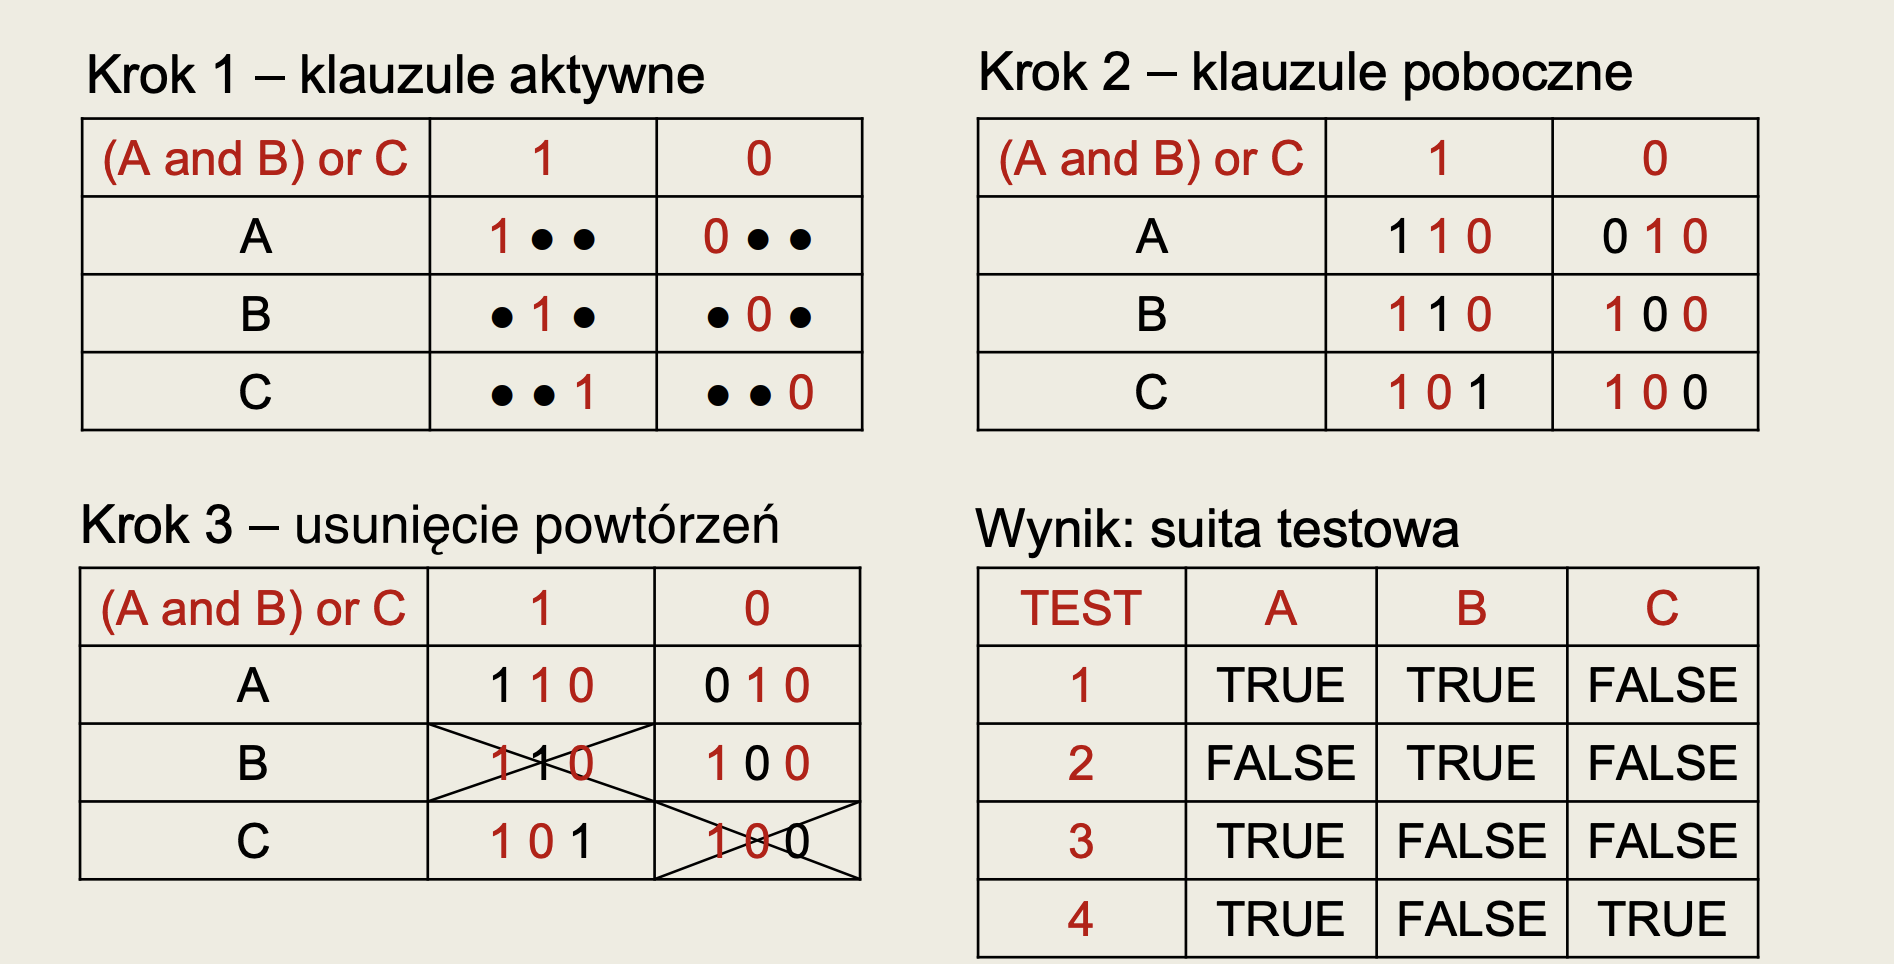
\includegraphics[width=\linewidth]{mcdc.png}
    \end{figure}

    \textbf{Zalety}
    \begin{itemize}
        \item dobre kryterium między słabym (C/D) i niepraktycznym (wiel. warunków)
        \item popularne w środowisku producentów awioniki (standard DO-178C)
        \item subsumuje pokrycie warunków/decyzji (dlaczego?), jednocześnie
        \item wymagając tylko liniowej względem liczby klauzul liczby testów
        \item dobra w znajdowaniu defektów takich jak:
        \begin{itemize}
            \item brakujący warunek, który powinien być obecny
            \item AND błędnie zaimplementowany jako OR i vice versa
            \item błędnie zaimplementowany operator relacyjny, np. < zamiast >
        \end{itemize}
        \item idea metody: wykryje błąd, gdy nastąpi błędne wartościowanie jednego(dowolnego!) z warunków decyzji
    \end{itemize}

    \textbf{Wady}
    \begin{itemize}
        \item problematyczne, jeśli występują tzw. termy powiązane (coupled terms)
        \begin{itemize}
            \item może się nie dać spełnić warunku MC/DC
            \item np. dla D = (A or B) and (not A) termy A i (not A) są powiązane
            \item żadna wartość B nie pozwala A być klauzulą aktywną
        \end{itemize}
        \item możliwe rozwiązania:
        \begin{itemize}
            \item wymagać kryterium MC/DC jedynie dla termów niepowiązanych
            \item analizować każdą decyzję zawierającą termy powiązane przypadek po przypadku
        \end{itemize}
        \item problem zwarcia (short-circuiting) może uniemożliwić osiągnięcie
        odpowiedniego pokrycia MC/DC
        \item bardziej skomplikowane niż słabsze kryteria
        \begin{itemize}
            \item na szczęście można znajdować testy automatycznie!
        \end{itemize}
    \end{itemize}

    \subsubsection{Problemy związane z pokryciem logicznym}

    \textbf{Problem sterowania} - jakie wartości x, y, z zadać, aby program wykonał się dokładnie taką ścieżką,
    jaką chcemy? Istnieją metody pomagające w tym, np. wykonanie symboliczne kodu (np. KLEE).

    \textbf{Problem zwarcia} - zwarcie to optymalizacja kompilatora pozwalająca szybciej ewaluować
    formuły logiczne (leniwa ewaluacja).

\end{document}
